\documentclass[a4paper,12pt]{article}

\usepackage[UTF8]{ctex}
\usepackage{geometry}
\usepackage{enumerate}
\usepackage{enumitem}
\usepackage{color}
\usepackage{graphics}


%%%%%%%%%%%%%%%%%%%%%%%%%%%%%%%%%%%
% Python 代码环境
%%%%%%%%%%%%%%%%%%%%%%%%%%%%%%%%%%%
\usepackage{listings}

\definecolor{dkgreen}{rgb}{0,0.6,0}
\definecolor{gray}{rgb}{0.5,0.5,0.5}
\definecolor{mauve}{rgb}{0.58,0,0.82}

\lstset{frame=tb,
  language=Python,
  aboveskip=3mm,
  belowskip=3mm,
  showstringspaces=false,
  columns=flexible,
  basicstyle={\small\ttfamily},
  numbers= left,
  numberstyle=\tiny\color{gray},
  keywordstyle=\color{blue},
  commentstyle=\color{dkgreen},
  stringstyle=\color{mauve},
  breaklines=true,
  breakatwhitespace=true,
  tabsize=3
}


%%%%%%%%%%%%%%%%%%%%%%%%%%%%%%%%%%%
% 页面版式设计
%%%%%%%%%%%%%%%%%%%%%%%%%%%%%%%%%%%
\geometry{scale=0.85}
\renewcommand{\labelenumi}{\arabic{enumi})}

\title{\bf 算法分析第三次作业}
\author{石发强\quad ZY1806707 \\
14061115@buaa.edu.cn \\
北京航空航天大学\quad 计算机学院}

\begin{document}
\maketitle
\section{题目}
用分支定界算法求以下问题:

某公司于乙城市的销售点急需一批成品,该公司成品生产基地在甲城市。甲城市与乙城市之间共有n座城市,互相以公路连通。甲城市、乙城市以及其它各城市之间的公路连通情况及每段公路的长度由矩阵M1给出。每段公路均由地方政府收取不同额度的养路费等费用,具体数额由矩阵M2给出。请给出在需付养路费总额不超过1500的情况下,该公司货车运送其产品从甲城市到乙城市的最短运送路线。

具体数据参见文件:
\begin{itemize}
    \item M1.txt
        
        各城市之间的公路连通情况及每段公路的长度矩阵(有向图),甲城市为城市Num.1,乙城市为城市Num.50
    \item M2.txt
        
        每段公路收取的费用矩阵(非对称)
\end{itemize}
\section{算法分析}
\subsection{算法流程}
\begin{enumerate}
    \item 读取所有城市间的距离矩阵m1和和代价矩阵m2
    \item 采用Floyd算法计算所有城市对之间的最短路径长度和最小代价,用于计算步骤\ref{process-4}中当前代价与当前距离
    \item 初始化一个栈,将0节点、即出发点甲城市压栈
    \item 取出栈顶节点,检查其所有相邻节点,确定下一个当前最优路径上的节点压栈;在检查的过程中如果发现超出最短路径或者代价限制1500,则进行剪枝(分支限界优化的核心步骤),然后弹栈回溯 \label{process-4}
    \item 找到一个解后,保存该解,然后重复步骤\ref{process-4},直到栈空,即可获得最优解
\end{enumerate}
\subsection{核心剪枝策略}
在算法流程步骤\ref{process-4}中剪枝的核心策略是当前路径超出当前最优路径或者当前代价超出当前最优代价,即
$$cur\_cost+mincost[cur][n-1] > cost\_bound\  or\  cur\_distance+mindist[cur] > distacne\_bound$$ 时则进行剪枝回溯,其中$n$为所有城市的个数。
\subsection{算法复杂度}
该实现算法中Floyd算法的时间复杂度为$O(n^3)$,而后进行DFS深度优先搜索的时间复杂度为$O(n+e)$,但是因为采取了分支限界的办法,所以实际的计算量会远小于$O(n+e)$,因此总的时间复杂度为{\color{red}$O(n^3)$},其中$n$是所有城市的个数、$e$所有城市间互相联通的有向图边的个数。

因为采用邻接矩阵的方式存储所有城市间的距离和联通性且没有其它空间开销,因此空间复杂度为{\color{red}$O(n^2)$},其中$n$是所有城市的个数。

\section{计算结果}
根据本题的具体数据,计算结果为从城市甲到城市乙:
\begin{itemize}
    \item 最短路径长度 \quad 464
    \item 养路费花费 \quad 1448
    \item 最短路径 \quad 1->3->8->11->15->21->23->26->32->37->39->45->47->50,需经过14个城市
    \item Python实现耗时约0.9s,cpp实现耗时在毫米级内。
\end{itemize}

\section{具体实现}
\subsection{Python实现}
代码文件见附件assignment\_2.py
\subsubsection{Python代码}
\begin{lstlisting}[language=Python]
    #!/usr/bin/env python
    # -*- coding:utf-8 -*-
    '''
    * @Author: shifaqiang(石发强)--[14061115@buaa.edu.cn] 
    * @Date: 2019-01-07 16:10:00 
    * @Last Modified by:   shifaqiang 
    * @Last Modified time: 2019-01-07 16:10:00 
    * @Desc: python implementation for algorithm analysis assignment_3
    '''

    import numpy as np
    import time

    def floyd(graph):
        '''
        from wikipad (https://en.wikipedia.org/wiki/Floyd%E2%80%93Warshall_algorithm),
        floyd algorithm is an method for finding shortest paths in a weighted graph 
        with positive or negative edge weights (but with no negative cycles).
        A single execution of the algorithm will find the lengths (summed weights) 
        of shortest paths between all pairs of vertices. 

        1 let dist be a |V| × |V| array of minimum distances initialized to ∞ (infinity)
        2 for each edge (u,v)
        3    dist[u][v] ← w(u,v)  // the weight of the edge (u,v)
        4 for each vertex v
        5    dist[v][v] ← 0
        6 for k from 1 to |V|
        7    for i from 1 to |V|
        8       for j from 1 to |V|
        9          if dist[i][j] > dist[i][k] + dist[k][j] 
        10             dist[i][j] ← dist[i][k] + dist[k][j]
        11         end if
        '''
        assert isinstance(graph, np.ndarray)
        # define 9999 as infinity
        n = graph.shape[0]
        for k in range(n):
            for i in range(n):
                for j in range(n):
                    graph[i][j] = min(graph[i][j], graph[i][k]+graph[k][j])
        return graph

    def dfs(distance, cost, mindist, mincost):
        """
        dfs with branch and bound
        """
        # check if parameters are legal
        assert isinstance(distance, np.ndarray) and isinstance(mindist, np.ndarray)
        assert isinstance(cost, np.ndarray) and isinstance(mincost, np.ndarray)
        assert distance.shape == cost.shape and distance.shape == mindist.shape
        assert cost.shape == mincost.shape
        # set some variable
        n = distance.shape[0]
        res = None
        # depth is the top of stack, cur is the current city, cur_next is the next feasible city of current city, visited is flag for all cities if they are visited
        stack, depth, cur, cur_next, visited = [0]*(n+2), 0, 0, 0, [False]*n
        # initialization of the dfs stack with start point city 0
        visited[0] = True
        # seting the bound
        cost_bound, distacne_bound, cur_distance, cur_cost = 1500, np.inf, 0, 0
        while depth >= 0:
            found, cur, cur_next = -1, stack[depth], stack[depth+1]
            for i in range(cur_next+1, n):
                # attempt all neighbor cities for city cur
                if distance[cur][i] == 9999 or visited[i]:
                    continue
                elif cur_cost+mincost[cur][n-1] > cost_bound or cur_distance+mindist[cur][n-1] > distacne_bound:
                    continue  # prune operation
                elif i < n:
                    found = i
                    break  # find a new feasible unvisited city, break the for loop
            if found == -1:
                # no feasible next city for cur city, backtracking
                depth -= 1
                cur_distance -= distance[stack[depth]][stack[depth+1]]
                cur_cost -= cost[stack[depth]][stack[depth+1]]
                visited[stack[depth+1]] = False
            else:
                # found a feasible next neighbor city for current city, update current path with cost, distance, path stack and visited record
                cur_cost += cost[stack[depth]][found]
                cur_distance += distance[stack[depth]][found]
                depth += 1
                stack[depth], stack[depth+1], visited[found] = found, 0, True
                if found == n-1:
                    # arrive at terminal city, found a new feasible solution
                    if cur_cost > 1500:
                        continue
                    res = stack[:depth+1], cur_cost, cur_distance
                    # update bound
                    distacne_bound = cur_distance
                    # backtracking
                    for i in range(2):
                        depth -= 1
                        cur_distance -= distance[stack[depth]][stack[depth+1]]
                        cur_cost -= cost[stack[depth]][stack[depth+1]]
                        visited[stack[depth+1]] = False
        return res

    if __name__ == "__main__":
        # load data
        start_time = time.time()
        distance = np.genfromtxt("m1.txt", skip_header=False, delimiter='\t', dtype=np.int32)
        cost = np.genfromtxt("m2.txt", skip_header=False, delimiter='\t', dtype=np.int32)
        assert distance.shape == cost.shape
        # compute result
        mindist = floyd(np.copy(distance))
        mincost = floyd(np.copy(cost))
        res = dfs(distance, cost, mindist, mincost)
        print("number of cities in best path:{}\nbest path:{}\nminimum cost:{}\nminimum distance:{}".format(len(res[0]), np.array(res[0])+1, res[1], res[2]))
        print("time cost:{}s".format(time.time()-start_time))
\end{lstlisting}
\subsubsection{Python运行结果}
经过分支限界优化,assignment\_2.py在1s内计算出了正确结果\footnote{评测所用机器配置为2 * Intel(R) Xeon(R) E5-2620 v3 @ 2.40GHz CPU},如图\ref{fig-python-result}所示。
\begin{figure}[h]
    \centering
    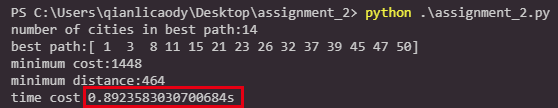
\includegraphics{./src/python_result.png}
    \caption{Python实现运行效果}
    \label{fig-python-result}
\end{figure}
\subsection{cpp实现}
\subsubsection{cpp实现代码}
代码文件见附件assignment\_2.cpp
\begin{lstlisting}[language=C]
    #include <stdio.h>
    #include <time.h>
    #include <iostream>
    #include <fstream>
    #include <regex>
    #include <string>
    #include <vector>
    #include <limits>

    using namespace std;
    struct record
    {
        int length; // number of cities
        vector<int> city;
        int minimum_cost;
        int minimum_dist;
    };
    #define size_t int

    void print(vector<vector<int>> &matrix)
    {
        // auxiliary output function
        for (auto i : matrix)
        {
            for (auto j : i)
                cout << j << " ";
            cout << endl;
        }
    }
    void load_matrix(string filename, vector<vector<int>> &matrix)
    {
        // load a 2-dimensions array to matrix from file filename
        vector<int> tmp;
        string line;
        ifstream in(filename);           //open file filename to ifstream
        regex pat_regex("[[:digit:]]+"); //match a type int number
        while (getline(in, line))
        {
            for (sregex_iterator it(line.begin(), line.end(), pat_regex), end_it; it != end_it; ++it)
            {
                tmp.push_back(stoi(it->str()));
            }
            matrix.push_back(tmp);
            tmp.clear();
        }
    }
    void floyd(vector<vector<int>> &graph)
    {
        int count = graph.size();
        for (size_t k = 0; k < count; k++)
            for (size_t i = 0; i < count; i++)
                for (size_t j = 0; j < count; j++)
                    graph[i][j] = min(graph[i][j], graph[i][k] + graph[k][j]);
    }
    record branch_and_bound(vector<vector<int>> &dist, vector<vector<int>> &cost, vector<vector<int>> &mindist, vector<vector<int>> &mincost)
    {
        /*
            depth is the top of stack, cur is the current city, cur_next is the next feasible city of current city, visited is flag for all cities if they are visited
        */
        int n = dist.size(), depth = 0;
        record res;
        int cost_bound = 1500, distance_bound = INT32_MAX, cur_distance = 0, cur_cost = 0;
        int *stack = new int[n + 2];
        bool *visited = new bool[n];
        memset(stack, 0, sizeof(int) * (n + 2));
        memset(visited, false, sizeof(bool) * n);
        visited[0] = true; //push first city 0 to stack and visit it
        while (true)
        {
            int found = -1, cur = stack[depth], cur_next = stack[depth + 1];
            for (size_t i = cur_next + 1; i < n; i++)
            {
                /* attempt all neighbor cities for city cur */
                if ((dist[cur][i] == 9999) || visited[i])
                    continue;
                else if ((cur_cost + mincost[cur][n - 1] > cost_bound) || (cur_distance + mindist[cur][n - 1] > distance_bound))
                    continue; // prune operation
                else if (i < n)
                {
                    found = i; // find a new feasible unvisited city i, break the for loop
                    // cout << "found city " << i << " for cur city " << cur << endl;
                    break;
                }
            }
            if (found == -1)
            {
                // no feasible next city for cur city, backtracking
                depth--;
                if (depth < 0)
                    break;
                cur_distance -= dist[stack[depth]][stack[depth + 1]];
                cur_cost -= cost[stack[depth]][stack[depth + 1]];
                visited[stack[depth + 1]] = false;
            }
            else
            {
                // found a feasible next neighbor city for current city, update current path with cost, distance, path stack and visited record
                cur_cost += cost[stack[depth]][found];
                cur_distance += dist[stack[depth]][found];
                depth++;
                stack[depth] = found, stack[depth + 1] = 0, visited[found] = true;
                if (found == n - 1)
                {
                    // arrive at terminal city, found a new feasible solution
                    if (cur_cost > 1500)
                        continue;
                    // update bound and record current best result
                    distance_bound = cur_distance;
                    res.length = depth + 1;
                    res.city.clear();
                    for (size_t i = 0; i < res.length; i++)
                        res.city.push_back(stack[i] + 1);
                    res.minimum_cost = cur_cost;
                    res.minimum_dist = cur_distance;
                    // backtracking for other feasible solution
                    for (size_t i = 0; i < 2; i++)
                    {
                        depth--;
                        cur_distance -= dist[stack[depth]][stack[depth + 1]];
                        cur_cost -= cost[stack[depth]][stack[depth + 1]];
                        visited[stack[depth + 1]] = false;
                    }
                }
            }
        }
        return res;
    }
    int main(int argc, char const *argv[])
    {
        time_t start = clock();
        // load data
        string dist_filename = "m1.txt", cost_filename = "m2.txt";
        vector<vector<int>> dist, cost, mindist, mincost;
        load_matrix(dist_filename, dist);
        mindist = dist;
        floyd(mindist);
        load_matrix(cost_filename, cost);
        mincost = cost;
        floyd(mincost);
        record res = branch_and_bound(dist, cost, mindist, mincost);
        cout << "number of cities in best path:" << res.length << "\nbest path:";
        for (size_t i = 0; i < res.length; i++)
            cout << res.city[i] << " ";
        cout << "\nminimum cost:" << res.minimum_cost << "\nminimum distance:" << res.minimum_dist << endl;
        cout << "time cost:" << (clock() - start) / double(CLOCKS_PER_SEC) << "s" << endl;
        return 0;
    }
\end{lstlisting}
\subsubsection{cpp运行结果}
经过分支限界优化,assignment\_2.exe在毫秒级时间内计算出正确结果,如图\ref{fig-cpp-result}所示。
\begin{figure}[htbp]
    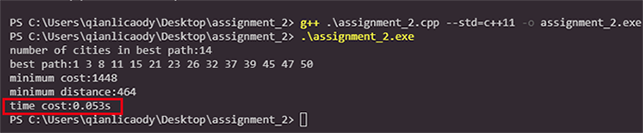
\includegraphics{./src/cpp_result.png}
    \caption{cpp实现运行效果}
    \label{fig-cpp-result}
\end{figure}
\section{附件}
\begin{enumerate}
    \item assignment\_2.py
    \item assignment\_2.cpp
    \item assignment\_2.exe\footnote{运行代码时请将Python代码文件或可执行文件与参数文件m1.txt、m2.txt置于同一目录下}
\end{enumerate}

\end{document}